% Running Time and Asymptotic Notation -- Metropolis beamer slides
% Compile: pdflatex -shell-escape? (not needed)  ->  pdflatex running-time.tex (x2)
\documentclass[10pt,aspectratio=169]{beamer}

\usetheme{metropolis}
\metroset{block=fill, numbering=fraction, progressbar=frametitle}

\usepackage[T1]{fontenc}
\usepackage{amsmath, amssymb}
\usepackage{listings}
\usepackage{booktabs}
\usepackage{tikz}
\usepackage{pgfplots}
\pgfplotsset{compat=1.18}
\usetikzlibrary{arrows.meta, positioning, decorations.pathreplacing, calc}

% ---- colors -------------------------------------------------------------
\definecolor{mLightBlue}{HTML}{4C72B0}
\definecolor{mGreen}{HTML}{55A868}
\definecolor{mRed}{HTML}{C44E52}
\definecolor{mGray}{HTML}{BFBFBF}
\setbeamercolor{alerted text}{fg=mRed}

% ---- code style ---------------------------------------------------------
\lstdefinestyle{jl}{
  basicstyle=\ttfamily\footnotesize,
  keywordstyle=\color{mRed}\bfseries,
  commentstyle=\color{mGreen}\itshape,
  numberstyle=\tiny\color{mGray},
  showstringspaces=false,
  breaklines=true,
  columns=fullflexible,
  morekeywords={function,for,in,if,end,return,length}
}
\lstset{style=jl}

% ---- array-drawing helper ----------------------------------------------
% \arrayrow{list of values}{index of min}{number of sorted cells}
\newcommand{\arrayrow}[3]{%
  \begin{tikzpicture}[scale=0.8, every node/.style={transform shape}]
    \foreach \v [count=\i from 0] in {#1} {
      \pgfmathtruncatemacro{\sorted}{#3}
      \pgfmathtruncatemacro{\mind}{#2}
      \ifnum\i<\sorted
        \def\fillc{mGreen!25}
      \else
        \ifnum\i=\mind \def\fillc{mRed!30}\else\def\fillc{black!5}\fi
      \fi
      \node[draw, minimum size=7mm, fill=\fillc] at (\i*0.75,0) {\small \v};
    }
  \end{tikzpicture}%
}

% ---- title --------------------------------------------------------------
\title{Running Time and Asymptotic Notation}
\subtitle{Data Structures \& Algorithms}
\date{}
\author{}

\begin{document}

\maketitle

% =========================================================================
\begin{frame}{Logistics}
  Grading scheme:

  \bigskip

  \begin{itemize}
    \item Homework 20\%
    \item In-class quizzes 20\% (2 lowest scores dropped)
    \item 2 exams 60\%
  \end{itemize}

  \pause

  \bigskip

  You will need a laptop or tablet for in-class quizzes or exams.
  Do not change browser tabs during quizzes or exams.  

  \pause 
   \bigskip

  All announcements, grades, and homework will be posted on Canvas. Check it regularly.



\end{frame}

% =========================================================================


\begin{frame}{Generative AI Usage Guidelines}


  \begin{itemize}
    \item Asking {\bf clarifying} questions related to lectures, homework, or exams is OK. Treat it as a tutor.
    \item For homework, you may use AI to do sanity checks on your solutions \bf{without} revealing the solution. See the syllabus for an example prompt.
  \end{itemize}

   The homework is only 20\% of your grade, so treat it as a learning opportunity.


\end{frame}



\begin{frame}{Generative AI Usage Guidelines}

  I do believe that AI is a powerful tool that can help you learn, but it is not a substitute for learning itself.

  \begin{alertblock}{My take} We will operate based on the premise that you believe in the value of learning. 
  \end{alertblock}

  \begin{itemize}
    \item Grow cognitive skills by doing the work yourself
    \item Understanding is important for both academic and professional success
    \item There is value in learning in itself
  \end{itemize}

\end{frame}

% =========================================================================
\begin{frame}{Algorithms}
  An algorithm is a \alert{precise, unambiguous} set of instructions that solves a problem.

  \bigskip
  Analyzing one has two parts:

  \pause
  \begin{itemize}
    \item Prove it is \alert{correct}.
    \item Evaluate its \alert{efficiency} --- time, memory, \ldots
  \end{itemize}


\end{frame}

% =========================================================================
\section{Running Time}

\begin{frame}[fragile]{Counting Instructions}
  Measure running time by the number of \alert{basic machine instructions}: memory accesses, pairwise arithmetic.

  \bigskip
  \begin{lstlisting}
A[i] = A[i] + 1
  \end{lstlisting}

  \bigskip
  \begin{center}
  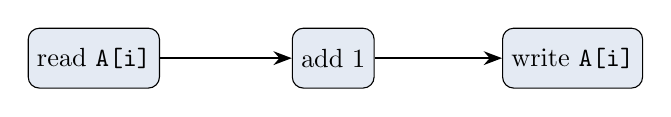
\begin{tikzpicture}[scale=0.95, every node/.style={transform shape}]
    \node[draw, rounded corners, fill=mLightBlue!15, minimum height=8mm] (r) at (0,0) {read \texttt{A[i]}};
    \node[draw, rounded corners, fill=mLightBlue!15, minimum height=8mm] (a) at (3.2,0) {add $1$};
    \node[draw, rounded corners, fill=mLightBlue!15, minimum height=8mm] (w) at (6.4,0) {write \texttt{A[i]}};
    \draw[-{Stealth}, thick] (r) -- (a);
    \draw[-{Stealth}, thick] (a) -- (w);
  \end{tikzpicture}
  \end{center}

  \bigskip
  \begin{center}
    Count instructions \alert{up to a constant factor}.
  \end{center}
\end{frame}

% =========================================================================
\begin{frame}{Selection Sort: The Idea}
  Scan \texttt{A[1:n]} for the smallest element, put it in \texttt{A[1]}.
  Then scan \texttt{A[2:n]}, put its smallest in \texttt{A[2]}. And so on.

  \bigskip
  \begin{center}
    \begin{tabular}{r@{\hskip 1em}l}
      $j=1$: & \arrayrow{5,2,9,1,7}{3}{0} \\[0.6em]
      $j=2$: & \arrayrow{1,2,9,5,7}{1}{1} \\[0.6em]
      $j=3$: & \arrayrow{1,2,9,5,7}{3}{2} \\[0.6em]
      $j=4$: & \arrayrow{1,2,5,9,7}{4}{3} \\[0.6em]
      done:  & \arrayrow{1,2,5,7,9}{-1}{5}
    \end{tabular}
  \end{center}

  \bigskip
  \begin{center}
    \small \textcolor{mGreen}{sorted prefix} \quad
    \textcolor{mRed}{minimum of the rest}
  \end{center}
\end{frame}

% =========================================================================
\begin{frame}[fragile]{Selection Sort}
  \begin{lstlisting}
function selection_sort!(A)
    n = length(A)                        # ln 1
    for j in 1:n-1                       # ln 2
        min_idx = j                      # ln 3
        for k in j+1:n                   # ln 4
            if A[min_idx] > A[k]         # ln 5
                min_idx = k              # ln 6
            end
        end
        A[j], A[min_idx] = A[min_idx], A[j]   # ln 7
    end
    return A
end
  \end{lstlisting}
\end{frame}

% =========================================================================
\begin{frame}{Counting the Lines}
  \begin{itemize}
    \item Lines 1, 2, 3 run $n-1$ times.
    \item Lines 4, 5, 6 run at most $(n-1)+(n-2)+\ldots+1$ times.
    \item Line 7 runs once.
  \end{itemize}

  \bigskip
  \begin{center}
  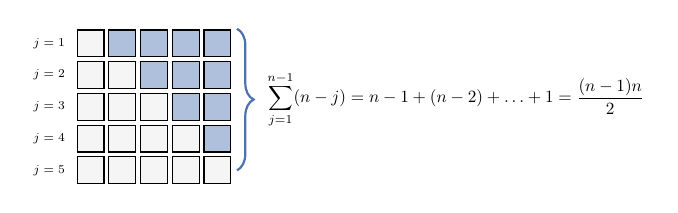
\begin{tikzpicture}[scale=0.62, every node/.style={transform shape}]
    \foreach \j in {1,...,5} {
      \foreach \k in {1,...,5} {
        \ifnum\k>\j
          \node[draw, fill=mLightBlue!45, minimum size=5.5mm] at (\k*0.65, -\j*0.65) {};
        \else
          \node[draw, fill=black!4, minimum size=5.5mm] at (\k*0.65, -\j*0.65) {};
        \fi
      }
      \node[left] at (0.25, -\j*0.65) {\scriptsize $j=\j$};
    }
    \draw[decorate, decoration={brace, amplitude=6pt}, mLightBlue, thick]
      (3.65,-0.35) -- (3.65,-3.25);
    \node[right] at (4.15,-1.8) {$\displaystyle \sum_{j=1}^{n-1}(n-j) =  n-1 + (n-2) + \ldots + 1 =
    \frac{(n-1)n}{2}$};
  \end{tikzpicture}
  \end{center}

  \bigskip
  Recall $1+2+\ldots+n = \dfrac{n(n+1)}{2}$.
  \pause 
  \begin{alertblock}{Total}
    $\displaystyle (n-1) + \frac{(n-1)n}{2} + 1 = O(n^2)$
  \end{alertblock}
\end{frame}

% =========================================================================
\begin{frame}{Growth}

  \begin{center}
  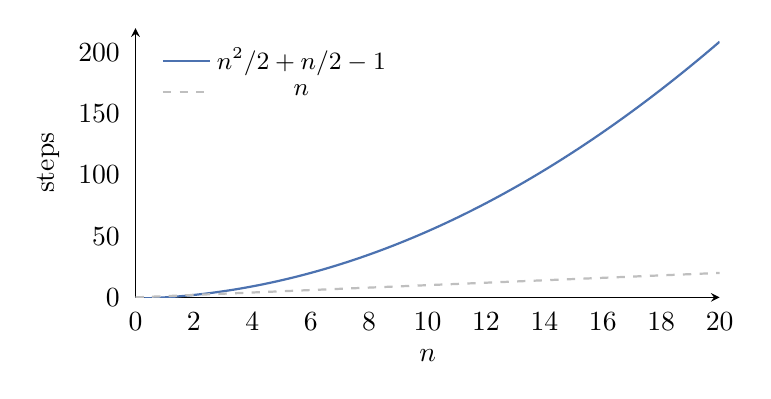
\begin{tikzpicture}
    \begin{axis}[
      width=9cm, height=5cm,
      xlabel={$n$}, ylabel={steps},
      domain=0:20, samples=100,
      legend pos=north west,
      legend style={draw=none, fill=none, font=\small},
      axis lines=left, tick style={draw=none},
      ymin=0, ymax=220,
    ]
      \addplot[thick, mLightBlue] {x*x/2 + x/2 - 1};
      \addlegendentry{$n^2/2 + n/2 - 1$}
      \addplot[thick, mGray, dashed] {x};
      \addlegendentry{$n$}
    \end{axis}
  \end{tikzpicture}
  \end{center}

  \begin{center}
    The running time grows \alert{quadratically} in $n$.
  \end{center}
\end{frame}

% =========================================================================
\begin{frame}[fragile]{Exercise}
  What is the running time of this function in terms of $n$?

  \begin{lstlisting}
function dummy_algorithm(n)
    for j in 1:n
        x = 0
        for k in 1:2^j
            y = 1
        end
    end
end
  \end{lstlisting}

  \begin{block}{Hint: geometric series}
    \[
      \sum_{i=0}^{m} r^i = \frac{r^{m+1}-1}{r-1}, \quad r \neq 1.
    \]
  \end{block}
\end{frame}

\begin{frame}{Solution}
  The inner loop runs $2^j$ times for each $j$. So the total work is
  \[
    \sum_{j=1}^{n} 2^j
    = \left(\sum_{j=0}^{n} 2^j\right) - 1
    = \frac{2^{n+1}-1}{2-1} - 1
    = 2^{n+1} - 2.
  \]

  \bigskip
  \begin{alertblock}{Answer}
    $O(2^n)$ --- the last iteration alone dominates everything before it.
  \end{alertblock}
\end{frame}

% =========================================================================
\section{Asymptotic Notation}

\begin{frame}{Why Asymptotics}
  For $T(n) = n^2/2 + n/2 - 1$, the term $n^2$ \alert{dictates} the growth.

  \bigskip
  \begin{center}
  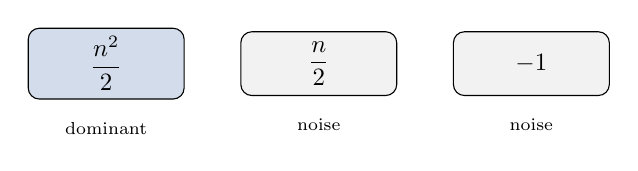
\begin{tikzpicture}[scale=0.9, every node/.style={transform shape}]
    \node[draw, rounded corners, fill=mLightBlue!25, minimum height=9mm, minimum width=22mm] (a) at (0,0) {$\dfrac{n^2}{2}$};
    \node[draw, rounded corners, fill=black!5, minimum height=9mm, minimum width=22mm] (b) at (3,0) {$\dfrac{n}{2}$};
    \node[draw, rounded corners, fill=black!5, minimum height=9mm, minimum width=22mm] (c) at (6,0) {$-1$};
    \node[below=2mm of a] {\scriptsize dominant};
    \node[below=2mm of b] {\scriptsize noise};
    \node[below=2mm of c] {\scriptsize noise};
  \end{tikzpicture}
  \end{center}

  \bigskip
  We write $f(n) = O(g(n))$ to say: $f$ grows \alert{no more} than $g$.
\end{frame}

% =========================================================================
\begin{frame}{Big-$O$}
  \begin{block}{Definition}
    $f(n) = O(g(n))$ if there exist constants $c > 0$ and $n_0$ such that
    \[
      f(n) \le c \cdot g(n) \quad \text{for all } n \ge n_0.
    \]
  \end{block}

  \bigskip
  \begin{center}
  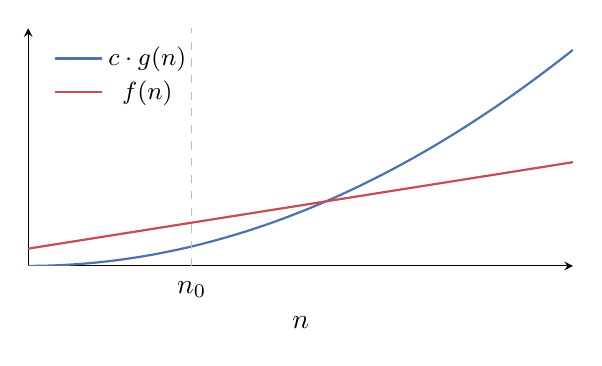
\begin{tikzpicture}
    \begin{axis}[
      width=8.5cm, height=4.6cm,
      domain=0:10, samples=100,
      axis lines=left, tick style={draw=none},
      xtick={3}, xticklabels={$n_0$}, ytick=\empty,
      xlabel={$n$},
      ymin=0, ymax=110, xmin=0, xmax=10,
      legend pos=north west,
      legend style={draw=none, fill=none, font=\small},
    ]
      \addplot[thick, mLightBlue] {x*x};
      \addlegendentry{$c\cdot g(n)$}
      \addplot[thick, mRed] {4*x + 8};
      \addlegendentry{$f(n)$}
      \draw[dashed, mGray] (axis cs:3,0) -- (axis cs:3,110);
    \end{axis}
  \end{tikzpicture}
  \end{center}
\end{frame}

% =========================================================================
\begin{frame}{Example}
  \begin{center}
    $3n^2 + 5n + 10 = O(n^2)$
  \end{center}

  \bigskip
  Take $c = 18$ and $n_0 = 1$. For $n \ge 1$:
  \[
    3n^2 + 5n + 10 \;\le\; 3n^2 + 5n^2 + 10n^2 \;=\; 18n^2.
  \]


\end{frame}

% =========================================================================
\begin{frame}{Example: $n^2 = O(1.5^n)$}
  Take $c = 1$ and $n_0 = 14$.

  \begin{center}
  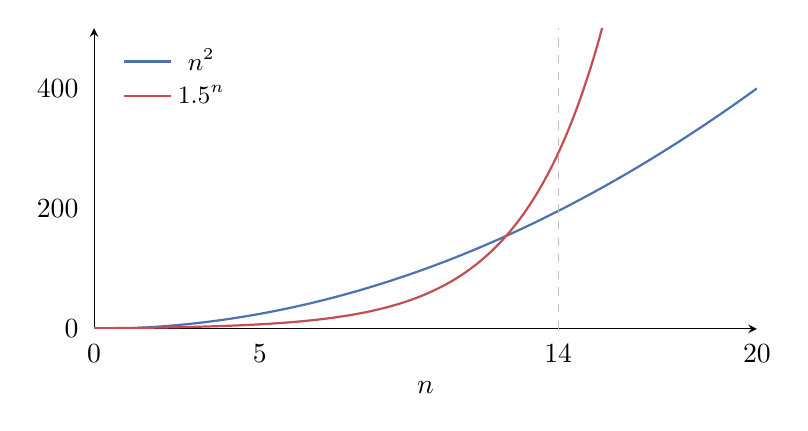
\begin{tikzpicture}
    \begin{axis}[
      width=10cm, height=5.4cm,
      domain=0:20, samples=200,
      axis lines=left, tick style={draw=none},
      xlabel={$n$},
      ymin=0, ymax=500, xmin=0, xmax=20,
      xtick={0,5,14,20},
      legend pos=north west,
      legend style={draw=none, fill=none, font=\small},
    ]
      \addplot[thick, mLightBlue] {x^2};
      \addlegendentry{$n^2$}
      \addplot[thick, mRed] {1.5^x};
      \addlegendentry{$1.5^n$}
      \draw[dashed, mGray] (axis cs:14,0) -- (axis cs:14,500);
    \end{axis}
  \end{tikzpicture}
  \end{center}
  \pause 
  \begin{center}
    From $n = 14$ onward, $n^2 \le 1.5^n$.
  \end{center}
\end{frame}

% =========================================================================
\begin{frame}{The Limit Approach}
  \begin{block}{}
    If $\displaystyle \lim_{n \to \infty} \frac{f(n)}{g(n)} = \text{constant} < \infty$, then $f(n) = O(g(n))$.
  \end{block}

  \bigskip
  \textbf{Example:}
  \[
    \lim_{n \to \infty} \frac{n^2/2 + n/2 - 1}{n^2}
    = \lim_{n \to \infty}\left(\frac{1}{2} + \frac{1}{2n} - \frac{1}{n^2}\right)
    = \frac{1}{2}.
  \]
\end{frame}

% =========================================================================
\begin{frame}{Example: $n + 10\ln n = O(n)$}
  \begin{center}
  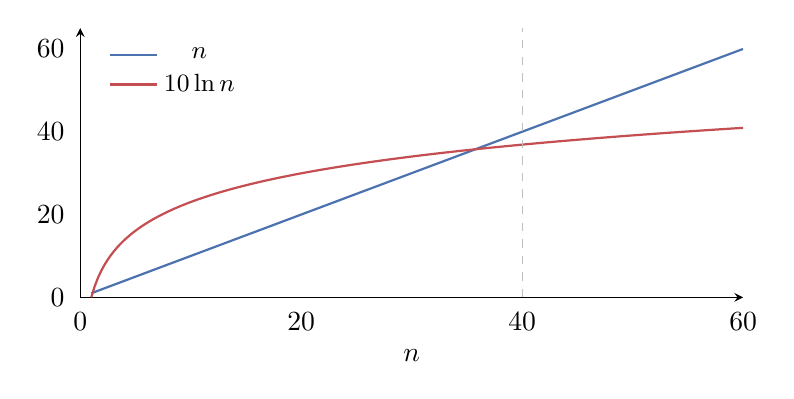
\begin{tikzpicture}
    \begin{axis}[
      width=10cm, height=5cm,
      domain=1:60, samples=200,
      axis lines=left, tick style={draw=none},
      xlabel={$n$},
      ymin=0, ymax=65, xmin=0, xmax=60,
      xtick={0,20,40,60},
      legend pos=north west,
      legend style={draw=none, fill=none, font=\small},
    ]
      \addplot[thick, mLightBlue] {x};
      \addlegendentry{$n$}
      \addplot[thick, mRed] {10*ln(x)};
      \addlegendentry{$10\ln n$}
      \draw[dashed, mGray] (axis cs:40,0) -- (axis cs:40,65);
    \end{axis}
  \end{tikzpicture}
  \end{center}

  For $n \ge 40$ we have $10 \ln n \le n$, hence
  \[
    n + 10\ln n \le n + n = 2n
    \qquad (c = 2,\ n_0 = 40).
  \]
\end{frame}

% =========================================================================
\begin{frame}{Same Example, via Limits}
  \begin{block}{L'H\^opital's rule}
    If $\lim f'(n)/g'(n)$ exists, then $\lim \dfrac{f(n)}{g(n)} = \lim \dfrac{f'(n)}{g'(n)}$.
  \end{block}

  \bigskip
  \[
    \lim_{n \to \infty} \frac{n + 10\ln n}{n}
    = \lim_{n \to \infty} \frac{1 + 10/n}{1}
    = 1 < \infty.
  \]
\end{frame}

% =========================================================================
\begin{frame}{Exercises}
  \begin{enumerate}
    \item Show that $\log_a n = O(\log_b n)$ for constants $a, b$.\\
      {\small Hint: change-of-base formula.}
    \bigskip
    \item Show that $2\sqrt{n} + n^{1/3}\log_2 n = O(\sqrt{n})$.
  \end{enumerate}
\end{frame}

\begin{frame}{Solution 1}
  Change of base: $\log_a n = \dfrac{\log_b n}{\log_b a}$.

  \bigskip
  Since $\log_b a$ is a \alert{constant}, take $c = 1/\log_b a$ and $n_0 = 1$:
  \[
    \log_a n = c \cdot \log_b n \le c \cdot \log_b n.
  \]

  \bigskip
  \begin{center}
    \small The base of a logarithm never matters inside $O(\cdot)$.
  \end{center}
\end{frame}

\begin{frame}{Solution 2}
  We need $n^{1/3}\log_2 n$ to be swallowed by $\sqrt{n} = n^{1/2}$:
  \[
    \frac{n^{1/3}\log_2 n}{n^{1/2}} = \frac{\log_2 n}{n^{1/6}} \xrightarrow[n \to \infty]{} 0,
  \]
  since a polynomial beats a logarithm.

  \bigskip
  So $n^{1/3}\log_2 n \le \sqrt{n}$ for large $n$, giving
  \[
    2\sqrt{n} + n^{1/3}\log_2 n \le 3\sqrt{n}
    \qquad (c = 3).
  \]
\end{frame}

% =========================================================================
\begin{frame}{Big-$\Omega$}
  \begin{block}{Definition}
    $g(n) = \Omega(f(n))$ if $f(n) = O(g(n))$.
  \end{block}

  \bigskip
  \begin{center}
  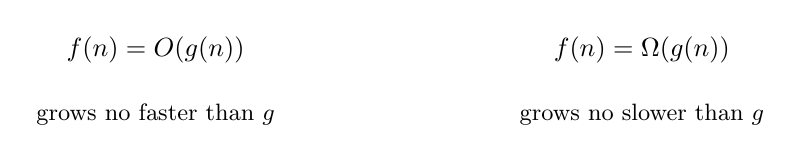
\begin{tikzpicture}[scale=0.95, every node/.style={transform shape}]
    \node (l) at (0,0) {$f(n) = O(g(n))$};
    \node (r) at (6.5,0) {$f(n) = \Omega(g(n))$};
    \node[below=3mm of l] {\small grows \alert{no faster} than $g$};
    \node[below=3mm of r] {\small grows \alert{no slower} than $g$};
  \end{tikzpicture}
  \end{center}
\end{frame}

% =========================================================================
\begin{frame}{Big-$\Theta$}
  \begin{block}{Definition}
    $f(n) = \Theta(g(n))$ if $f(n) = O(g(n))$ \emph{and} $g(n) = O(f(n))$.
  \end{block}

  \bigskip
  Equivalently, via limits:
  \[
    0 < \lim_{n \to \infty}\frac{f(n)}{g(n)} < \infty.
  \]

  \bigskip
  \begin{center}
    Neither function grows strictly faster than the other.
  \end{center}
\end{frame}

\begin{frame}{Example: $2n^{100} + n^{99} = \Theta(n^{100})$}
  \[
    \lim_{n \to \infty} \frac{2n^{100} + n^{99}}{n^{100}} = 2
    \qquad\Longrightarrow\qquad
    2n^{100} + n^{99} = O(n^{100}).
  \]

  \bigskip
  \[
    \lim_{n \to \infty} \frac{n^{100}}{2n^{100} + n^{99}}
    = \lim_{n \to \infty}\frac{1}{2 + 1/n} = \frac{1}{2}
    \quad\Longrightarrow\quad
    n^{100} = O(2n^{100} + n^{99}).
  \]

  \bigskip
  Both directions hold, so the two functions have the \alert{same growth}.
\end{frame}

% =========================================================================
\begin{frame}{Exercises}
  \begin{enumerate}
    \item Show that $n^{1.99} = O(n^2)$ but $n^{1.99} \neq \Theta(n^2)$.
    \bigskip
    \item Show that if $n$ is a power of $2$, then
      $2 + 4 + 8 + \ldots + n = \Theta(n)$.
  \end{enumerate}
\end{frame}

\begin{frame}{Solution 1}
  \textbf{Upper bound.} $\displaystyle \lim_{n\to\infty}\frac{n^{1.99}}{n^2} = \lim_{n\to\infty} n^{-0.01} = 0 < \infty$,
  so $n^{1.99} = O(n^2)$.

  \bigskip
  \textbf{Not $\Theta$.} For $\Theta$ we would also need $n^2 = O(n^{1.99})$, but
  \[
    \lim_{n\to\infty}\frac{n^2}{n^{1.99}} = \lim_{n\to\infty} n^{0.01} = \infty.
  \]

  \bigskip
  No constant $c$ can satisfy $n^2 \le c\, n^{1.99}$ for all large $n$. In fact $n^{1.99} = o(n^2)$.
\end{frame}

\begin{frame}{Solution 2}
  Write $n = 2^m$. The sum is a geometric series:
  \[
    2 + 4 + \ldots + 2^m
    = \left(\sum_{i=0}^{m} 2^i\right) - 1
    = \frac{2^{m+1}-1}{2-1} - 1
    = 2 \cdot 2^m - 2 = 2n - 2.
  \]

  \bigskip
  Since $n \le 2n - 2 \le 2n$ for $n \ge 2$, the sum is $\Theta(n)$.

  \bigskip
  \begin{center}
    \small A doubling sum is dominated by its \alert{last} term.
  \end{center}
\end{frame}

% =========================================================================
\begin{frame}{Little-$o$ and Little-$\omega$}
  \begin{block}{Definition}
    $f(n) = o(g(n))$ if for \emph{any} constant $c > 0$ there is $n_0$ with
    $f(n) < c \cdot g(n)$ for all $n \ge n_0$.
    \quad Equivalently $\displaystyle \lim_{n\to\infty}\frac{f(n)}{g(n)} = 0$.
  \end{block}

  \begin{block}{Definition}
    $f(n) = \omega(g(n))$ if $g(n) = o(f(n))$.
    \quad Equivalently $\displaystyle \lim_{n\to\infty}\frac{f(n)}{g(n)} = \infty$.
  \end{block}

  \bigskip
  \begin{center}
    \alert{Strictly} slower and \alert{strictly} faster growth.
  \end{center}
\end{frame}

\begin{frame}{Examples}
  \textbf{Claim:} $\log_2 n = o(n^{0.1})$.
  \[
    \lim_{n\to\infty}\frac{\log_2 n}{n^{0.1}}
    = \frac{1}{\ln 2}\lim_{n\to\infty}\frac{\ln n}{n^{0.1}}
    = \frac{1}{\ln 2}\lim_{n\to\infty}\frac{1/n}{0.1\, n^{-0.9}}
    = \frac{1}{\ln 2}\lim_{n\to\infty}\frac{10}{n^{0.1}} = 0.
  \]

  \bigskip
  \textbf{Claim:} $3^n = \omega(2^n)$.
  \[
    \lim_{n\to\infty}\frac{3^n}{2^n} = \lim_{n\to\infty}(3/2)^n = \infty.
  \]
\end{frame}

% =========================================================================
\begin{frame}{Recap}
  \begin{center}
  \begin{tabular}{ll}
    \toprule
    $f(n) = O(g(n))$      & growth \alert{at most} $g$ \\
    $f(n) = \Omega(g(n))$ & growth \alert{at least} $g$ \\
    $f(n) = \Theta(g(n))$ & growth the \alert{same} as $g$ \\
    $f(n) = o(g(n))$      & growth \alert{strictly slower} than $g$ \\
    $f(n) = \omega(g(n))$ & growth \alert{strictly faster} than $g$ \\
    \bottomrule
  \end{tabular}
  \end{center}

  \bigskip
  \begin{center}
  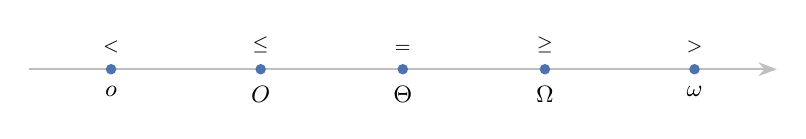
\begin{tikzpicture}[scale=0.95, every node/.style={transform shape}]
    \draw[-{Stealth}, thick, mGray] (-0.5,0) -- (9.5,0);
    \node[below=1mm] at (0.6,0) {\small $o$};
    \node[below=1mm] at (2.6,0) {\small $O$};
    \node[below=1mm] at (4.5,0) {\small $\Theta$};
    \node[below=1mm] at (6.4,0) {\small $\Omega$};
    \node[below=1mm] at (8.4,0) {\small $\omega$};
    \foreach \x in {0.6,2.6,4.5,6.4,8.4} \fill[mLightBlue] (\x,0) circle (2pt);
    \node[above=1mm] at (0.6,0) {\scriptsize $<$};
    \node[above=1mm] at (2.6,0) {\scriptsize $\le$};
    \node[above=1mm] at (4.5,0) {\scriptsize $=$};
    \node[above=1mm] at (6.4,0) {\scriptsize $\ge$};
    \node[above=1mm] at (8.4,0) {\scriptsize $>$};
  \end{tikzpicture}
  \end{center}
\end{frame}

% =========================================================================
\section{Useful Facts}

\begin{frame}{Fact 1: Polynomials}
  A polynomial grows like its \alert{most significant term}:
  \[
    3n^3 - n^2 + 100n = \Theta(n^3).
  \]

  \bigskip
  A polynomial always beats a poly-logarithm:
  \[
    \begin{aligned}
      n           &= \omega(\log^{999} n), \\
      n^{0.1}     &= \omega(\log^{99} n), \\
      n \log^2 n  &= o(n^{1.01}).
    \end{aligned}
  \]
\end{frame}

\begin{frame}{Fact 2: Exponentials}
  An exponential (base $> 1$) always beats a polynomial:
  \[
    \begin{aligned}
      n^{99} &= o(2^n), \\
      n^{10} &= o(1.01^{2n}).
    \end{aligned}
  \]

  \bigskip
  \begin{center}
  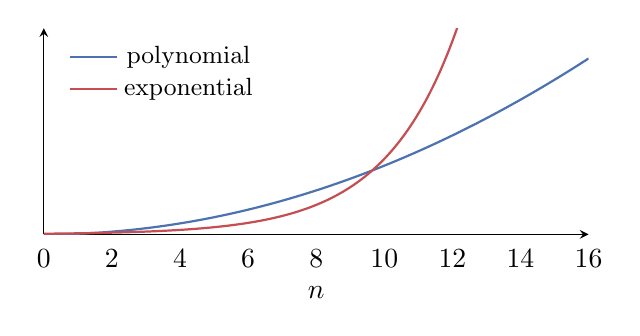
\begin{tikzpicture}
    \begin{axis}[
      width=8.5cm, height=4.2cm,
      domain=0:16, samples=200,
      axis lines=left, tick style={draw=none},
      xlabel={$n$}, ytick=\empty,
      ymin=0, ymax=300, xmin=0, xmax=16,
      legend pos=north west,
      legend style={draw=none, fill=none, font=\small},
    ]
      \addplot[thick, mLightBlue] {x^2};
      \addlegendentry{polynomial}
      \addplot[thick, mRed] {1.6^x};
      \addlegendentry{exponential}
    \end{axis}
  \end{tikzpicture}
  \end{center}
\end{frame}

% =========================================================================
\begin{frame}{Fact 3: Power Sums}
  \begin{block}{}
    For any constant $c$: \quad $1^c + 2^c + \ldots + n^c = \Theta(n^{c+1})$.
  \end{block}

  \bigskip
  \textbf{Upper bound.} Every term is at most $n^c$:
  \[
    1^c + 2^c + \ldots + n^c
    \le \underbrace{n^c + n^c + \ldots + n^c}_{n \text{ times}}
    = n^{c+1}.
  \]

  \bigskip
  \begin{center}
    So the sum is $O(n^{c+1})$. The lower bound needs more work.
  \end{center}
\end{frame}

\begin{frame}{Approximation by Integrals}
  \begin{center}
  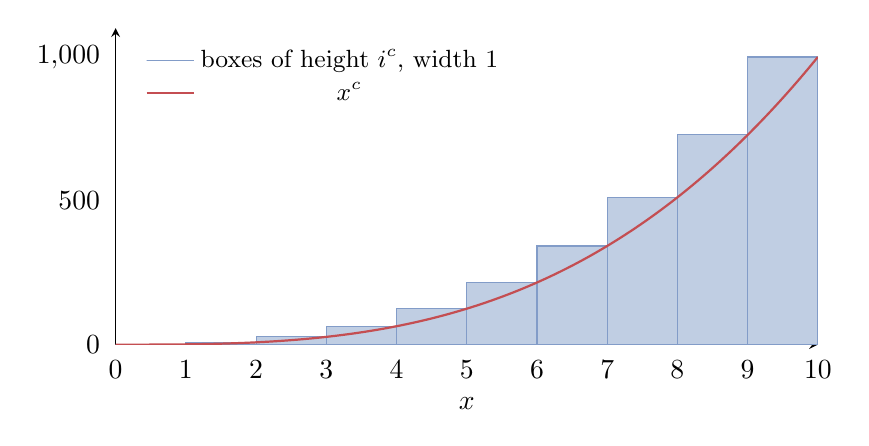
\begin{tikzpicture}
    \begin{axis}[
      width=10.5cm, height=5.6cm,
      axis lines=left, tick style={draw=none},
      xlabel={$x$}, ylabel={},
      xmin=0, xmax=10, ymin=0, ymax=1100,
      xtick={0,1,2,3,4,5,6,7,8,9,10},
      legend pos=north west,
      legend style={draw=none, fill=none, font=\small},
    ]
      \addplot[ybar interval, fill=mLightBlue!35, draw=mLightBlue!70]
        coordinates {(0,1)(1,8)(2,27)(3,64)(4,125)(5,216)(6,343)(7,512)(8,729)(9,1000)(10,1000)};
      \addlegendentry{boxes of height $i^c$, width $1$}
      \addplot[thick, mRed, domain=0:10, samples=200] {x^3};
      \addlegendentry{$x^c$}
    \end{axis}
  \end{tikzpicture}
  \end{center}

  \begin{center}
    \small Box area $= 1^c + 2^c + \ldots + n^c$ \ $\ge$ \ area under the curve.
  \end{center}
\end{frame}

\begin{frame}{Fact 3: Lower Bound}
  Each box at position $i$ has width $1$ and height $i^c$, so the boxes cover the curve:
  \[
    1^c + 2^c + \ldots + n^c
    \;\ge\; \int_0^n x^c \, dx
    \;=\; \frac{n^{c+1}}{c+1}.
  \]

  \bigskip
  Hence the sum is $\Omega(n^{c+1})$, and combined with the upper bound,
  \[
    1^c + 2^c + \ldots + n^c = \Theta(n^{c+1}).
  \]

  \bigskip
  \begin{center}
    \small E.g. $1^2 + 2^2 + \ldots + n^2 = \Theta(n^3)$.
  \end{center}
\end{frame}

% =========================================================================
\begin{frame}{Facts 4 and 5}
  \begin{block}{Fact 4}
    For any constant $c$, \quad $c = O(1)$.
  \end{block}

  \bigskip
  \begin{block}{Fact 5}
    If $a < b$, then $a^n = o(b^n)$. \quad E.g. $2^n = o(3^n)$.
  \end{block}
\end{frame}

% =========================================================================
\begin{frame}{A Common Pitfall}
  The following proof is \alert{wrong}:
  \[
    1 + 2 + 3 + \ldots + n = O(1) + O(1) + \ldots + O(1) = O(n).
  \]

  \bigskip
  But we know $1 + 2 + \ldots + n = \dfrac{n(n+1)}{2} = \Theta(n^2)$.

  \bigskip
  \begin{alertblock}{What went wrong}
    For a \emph{fixed} $i$, yes, $i = O(1)$.\\
    Inside $\sum_{i=1}^{n} i$, the value $i$ ranges up to $n$ --- it is \alert{not} a constant.
  \end{alertblock}

  \bigskip
  \begin{center}
    \small Be careful with sums whose number of terms is not fixed.
  \end{center}
\end{frame}



\end{document}
